\documentclass[pagesize=auto]{scrartcl}

\usepackage{fixltx2e}
\usepackage{etex}
\usepackage{lmodern}
\usepackage[T1]{fontenc}
\usepackage{textcomp}
\usepackage{amstext}
\usepackage{array}
\usepackage{xcolor}
\usepackage{tikz}
\usepackage{microtype}
\usepackage{hyperref}

\newcommand*{\mail}[1]{\href{mailto:#1}{\texttt{#1}}}
\newcommand*{\pkg}[1]{\textsf{#1}}
\newcommand*{\cls}[1]{\textsf{#1}}
\newcommand*{\cs}[1]{\texttt{\textbackslash#1}}
\makeatletter
\newcommand*{\cmd}[1]{\cs{\expandafter\@gobble\string#1}}
\makeatother
\newcommand*{\env}[1]{\texttt{#1}}
\newcommand*{\opt}[1]{\texttt{#1}}
\newcommand*{\meta}[1]{\textlangle\textsl{#1}\textrangle}
\newcommand*{\marg}[1]{\texttt{\{}\meta{#1}\texttt{\}}}
\newcommand*{\oarg}[1]{\texttt{[}\meta{#1}\texttt{]}}

\addtokomafont{title}{\rmfamily}

\title{The \pkg{wrapfig} package\thanks{This manual corresponds to \pkg{wrapfig.sty}~v3.6, dated~Jan 31, 2003.}}
\author{Donald Arseneau\thanks{\mail{asnd@triumf.ca}}}
\date{Jan 31, 2003}


\begin{document}

\maketitle

\noindent
\pkg{Wrapfig.sty} provides the environments \env{wrapfigure} and \env{wraptable} for
typesetting a narrow float at the edge of the text, and making the text
wrap around it.  The \env{wrapfigure} and \env{wraptable} environments interact
properly with the \cmd{\caption} command to produce proper numbering, but
they are not regular floats like \env{figure} and \env{table}, so (beware!) they
may be printed out of sequence with the regular floats.  There are four
parameters for \verb+\begin{wrapfigure}+, two optional and two required, plus
the text of the figure, with a caption perhaps:
%
\begin{quote}
  \verb+\begin{wrapfigure}[12]{r}[34pt]{5cm}+ \meta{figure} \verb+\end{wrapfigure}+\\
  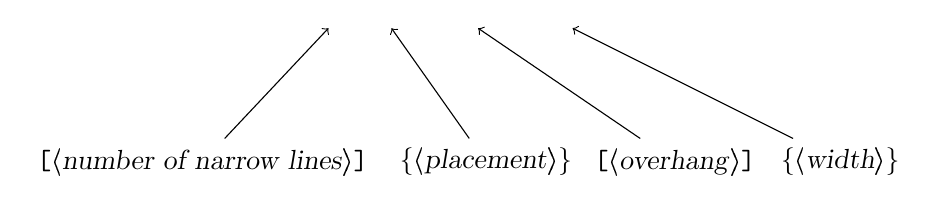
\begin{tikzpicture}
    \node (number) at (0mm, 0mm) {\oarg{number of narrow lines}};
    \node (placement) at (36mm, 0mm) {\marg{placement}};
    \node (overhang) at (60mm, 0mm) {\oarg{overhang}};
    \node (width) at (81mm, 0mm) {\marg{width}};
    \begin{scope}[->]
      \draw (number) -- (16mm, 17mm);
      \draw (placement) -- (24mm, 17mm);
      \draw (overhang) -- (35mm, 17mm);
      \draw (width) -- (47mm, 17mm);
    \end{scope}
  \end{tikzpicture}
\end{quote}


Some idiosyncrasies:
%
\begin{itemize}
\item You must not specify a \env{wrapfigure} in any type of list environment or
  or immediately before or immediately after one.  It is OK to follow
  a list if there is a blank line (\cs{par}) in between.

\item If you put a \env{wrapfigure} in a \env{parbox} or a \env{minipage}, or any other type
  of grouping, the text wrapping should end before the group does.

\item It does work in two-column format, but are your figures that small?

\item It may be out of sequence with regular floats.

\item The hlines that may be printed above and below floats are ignored;
  you must insert them manually if desired.

\item \cmd{\linewidth} is now adjusted within the wrapped text, but since it
  can only be set for whole paragraphs at a time, it will persist with
  the wrong value after the wrapping, until the paragraph is finished.
\end{itemize}

New wrapping environments may be added when new float types are defined
(using \cls{memoir.cls}, \pkg{float.sty}, or \pkg{ccaption.sty}).  Any wrapping environment,
\env{wrapfigure}, \env{wraptable}, or something else may be invoked using the
\env{wrapfloat} environment, as in \verb+\begin{wrapfloat}{figure}{O}{5cm}+.

To use \pkg{float.sty} properly, load package \pkg{float} before \pkg{wrapfig}, 
and declare any new float types after loading both.  Likewise for
\pkg{ccaption.sty} and \cmd{\newfloatlist} and \pkg{memoir.cls} and its \cmd{\newfloat}.


\section{Placement and Floating}

Parameter \verb+#2+ (required) is the figure placement code, but the valid
codes are different from regular figures.  They come in pairs: an
uppercase version which allows the figure to float, and a lowercase
version that puts the figure ``exactly here''.
%
\begin{quote}
  \begin{tabular}{*{2}{>{\ttfamily}l}!{--}l}
    r & R & the right side of the text                                      \\
    l & L & the left side of the text                                       \\
    i & I & the inside edge--near the binding (if \opt{[twoside]} document) \\
    o & O & the outside edge--far from the binding
  \end{tabular}
\end{quote}
%
You should specify one code only, not a list.  The figure or table must
be on one side or the other; it cannot be in the middle with text on
both sides.  The \texttt{i} and \texttt{o} options refer to the inside and outside of
the whole page, not individual columns.

The ability to float is somewhat restricted, and you will get best results
by giving exact manual placement, but floating is more convenient while
revising the document.  Any changes to the formatting can ruin your manual
positioning so you should adjust the placement just before printing a
final copy.  Here are some tips for good placement:
%
\begin{itemize}
\item The environment should be placed so as to not run over a page break.

\item The environment must not be placed in special places like lists.

\item For esthetic reasons, only plain text should wrap around the figure.
  Section titles and big equations look bad; lists are bad if the figure 
  is on the left.  (All these function properly, they just don't look 
  very good.)  Small equations look fine.

\item It is convenient to begin the environment between paragraphs, but if
  you want placement in the middle of a paragraph, you must put the
  environment between two words where there is a natural line break.
\end{itemize}

When floating, \LaTeX\ tries to apply these rules.  More specifically,
a floated wrapping environment will only begin\dots
%
\begin{itemize}
\item at the beginning of a paragraph,

\item when there is enough room on the page, or it is possible to go on
  the next page,

\item if the `paragraph' is not in a section title or a list,

\item if the paragraph is not wrapping around another figure,

\item in the main text (not in a \env{minipage} etc.)
\end{itemize}

It is possible that a non-floating \env{wrapfigure} will be forced to float
when an earlier one is still being processed.  A warning will be written
in that case.  You can have more information about the floating process
written to the log file by specifying \verb+\usepackage[verbose]{wrapfig}+.

If there is a lot of flexibility on a page, a floating \env{wrapfigure} may
be placed badly; you must turn to manual placement.  A rare problem is
that floats and footnotes specified within the wrapping text can also
cause poor placement and bad formatting.


\section{Sizing and optional overhang}

Parameter \verb+#4+ (the second required parameter) is the width of the figure
or table.  Given the way that \LaTeX\ puts just about everything into boxes 
with the current line-width, the width parameter will take precedence over 
whatever natural width the figure has.  In particular, the caption is always 
typeset with the specified width.  If the figure is wider than the space 
allotted, you will get an ``overfull box'' warning.

However, if you specify a width of \emph{zero} (\texttt{0pt}), the actual width of
the figure will determine the wrapping width.  A following \cmd{\caption}
should have the same width as the figure, but it might fail badly; it
is safer to specify a width when you use a caption.

\LaTeX\ will wrap surrounding text around the figure, leaving a gap of
\cmd{\intextsep} at the top and bottom, and \cmd{\columsep} at the side, by
producing a series of shortened text lines beside the figure.  The
indentation (shortening) of the text is the figure width plus \cmd{\columnsep}
minus overhang (if any; see below).

\LaTeX\ calculates the number of short lines needed based on the height
of the figure and the length \cmd{\intextsep}.  You can override this guess
by giving the first optional argument (parameter \verb+#1+) specifying the
number of shortened lines (counting each displayed equation as 3~lines).
This is particularly useful when the surrounding text contains extra
vertical spacing that is not accounted for automatically.

The second optional parameter (\verb+#3+) tells how much the figure should
hang out into the margin. The default overhang is given by the length
\cmd{\wrapoverhang}, which is \texttt{0pt} normally but can be changed using
\cmd{\setlength}.  For example, to have all wrapfigures use the space
reserved for marginal notes,
%
\begin{verbatim}
    \setlength{\wrapoverhang}{\marginparwidth}
    \addtolength{\wrapoverhang}{\marginparsep}
\end{verbatim}

When you do specify the overhang explicitly for a particular figure, you
can use a special unit called \cmd{\width} meaning the width of the figure.
For example, \verb+[0.5\width]+ makes the center of the figure sit on the
edge of the text, and \verb+[\width]+ puts the figure entirely in the margin
(and the adjacent text is indented by just \cmd{\columnsep}).  This \cmd{\width}
is the actual width of the \env{wrapfigure}, which may be greater than the 
declared width.


\section{Some Random Implementation Notes}

Unfortunately, \LaTeX's system of setting \cmd{\everypar} and \cs{par} is
unable to coexist peacefully with a wrapping environment, so I was
forced to subvert the \cmd{\@setpar} mechanism and \cmd{\everypar}.  (\cmd{\everypar}
is already subverted once by NFSS.)

When checking the room left on the page, remember that if there is less
than \cmd{\baselineskip} the new paragraph will begin on the next page, even
if there is no page stretch. If non-floating, I force a bad page break
rather than have the figure hang into the bottom margin.

Here are notes on various variables and some macros; what info they
store and how they are used.
%
\begin{description}
\item[\cmd{\WF@wli}] number-of-wrapped-lines parameter, saved for start of wrapping.
  Set globally by \cmd{\WF@wr} (set empty if no optional parameter given).
  The floating mechanism ignores this and uses the real size.

\item[\cmd{\WF@ovh}] margin overhang set globally by \cmd{\WF@rapt}, saved until placing
  figure (but not reset).  Actually, the setting is very tricky so that
  the expected values are used when a figure floats. First, the expression
  is saved without evaluation by \cmd{\WF@rapt} (\verb+\begin{wrapfigure}+) because
  \cmd{\width} is still unknown.  Soon after that, \cmd{\endwrapfigure} executes
  \cmd{\WF@ovh} to evaluate the overhang and save the result (so that changes
  to \cmd{\wrapoverhang} while this figure is floating won't affect this
  figure). Finally, it is used by \cmd{\WF@putfigmaybe} when printing the fig.

\item[\cmd{\WF@place}] a macro that is used as a number, giving the placement code.
  It might start out as \texttt{\textasciigrave I} and later be converted to \texttt{114} (r).

\item[\cmd{\WF@box}] tested for void at \verb+\begin{wrapfigure}+, to avoid collisions, % \end{wrapfigure}
  by \cmd{\everypar} to do floating, and by \cmd{\WF@finale} before resetting
  \cmd{\everypar}.  Voided globally when used by \cmd{\WF@putfigmaybe} (or by
  \cmd{\WF@wr} if an old figure must be dumped prematurely).

\item[\cs{par}] test if it is \cmd{\@@par} by \verb+\begin{wrapfigure}+ and \cmd{\WF@floathand} % \end{wrapfigure}
  to float past special environments.  It is set to \cmd{\@par} (\cmd{\WF@mypar})
  by \cmd{\WF@startwrapping}, and restored by an end-group (bad!)\ or by
  \cmd{\WF@finale} (good).  It is protected from change by redefining
  \cmd{\@setpar}.

\item[\cmd{\parshape}] let to \cmd{\WF@fudgeparshape} by \cmd{\WF@startwrapping}, so lists
  will continue wrapping; \cmd{\@@parshape} preserves the real \cmd{\parshape}
  command, and it is restored by \cmd{\WF@finale} or \cmd{\@parboxrestore}.
  \cmd{\WF@floathand} and \cmd{\WF@wr} test if old wrapping is still in progress
  with \verb+\ifx\parshape\WF@fudgeparshape+. The value of \cmd{\@@parshape} is
  also tested to float past lists and other wrapping environments.

\item[\cmd{\hangindent}] tested to float past section titles etc.

\item[\cmd{\c@WF@wrappedlines}] $\text{the number of shortened lines} + 1$; set globally by
  \cmd{\WF@start\-wrapping} and decremented by \cs{par} (\cmd{\WF@mypar}).  It is $> 1$
  only when wrapping is incomplete.  \cmd{\WF@wraphand}, \cmd{\WF@fudgeparshape},
  and \cmd{\WF@mypar} test the number for calling \cmd{\WF@finale}.  It may get
  stuck at some high value if \cs{par} is restored by an end-group, (and
  wrapping is terminated prematurely) so it is unwise to use this as a
  test for wrapping-complete.

\item[\cmd{\pagetotal}] one of many parameters used to compute floating.  When
  putting a \env{wrapfigure} in a \env{parbox}, I assign \verb+\let\pagetotal\maxdimen+
  (locally!)\ to signal not-top-of-page and no floating.

\item[\cmd{\WF@pspars}] the \cmd{\parshape} parameters as \LaTeX\ sets them for lists
  (\cmd{\WF@fudgepar\-shape}); when wrapping I test it and use it to modify my
  own real params for the paragraph.  They are also used when \cmd{\parshape}
  is restored after wrapping.

\item[\cmd{\WF@finale}] is performed by \cs{par} when wrapping should end.  However,
  that might happen inside a group (a list especially), so the subverted
  versions of \cs{par}, \cmd{\parshape} etc. will be reinstated when the group
  ends.  Thus, they must themselves test $\text{\cmd{\c@WF@wrappedlines}} < 2$ to see
  when wrapping is over, and if so, they should just do \cmd{\WF@finale} again.
\end{description}

These are the tests to see if a floating \env{wrapfigure} will fit at a particular
spot.  These tests are performed at the beginning of every paragraph after
the figure, except in lists etc.  ($\text{\cmd{\pagegoal}} - \text{\cmd{\pagetotal}}$ is the room
left on the page.)
%
\begin{verbatim}
  >
  room_left := \pagegoal - \pagetotal
  if  room_left < 0  then page overfull already:
     put figure (on next page)
  else
     if  figure_size > room_left  then does not fit
        if  max(min_stretch, \pagestretch) + extra > room_left
           then page can stretch until full: 
               put figure (at top of next page)
        fi
     else figure fits: put figure
  fi fi
  <
\end{verbatim}

Even if a \env{wrapfigure} is not floating, it will go through the same logic
to generate a \cmd{\pagebreak}, and maybe an underfull page, when the current
page can stretch until full.  The \texttt{min\_stretch} depends on whether it is
floating or not: \verb+.5\baselineskip+ (floating) \verb+2\baselineskip+ (not). The
\texttt{extra} is \verb+.5\baselineskip+ in either case.  These values can be adjusted.

There are some other `magic numbers' for floating that aren't really so
special, but you must change them together if you change them at all.
To make floating wrapfigures float less and fit on pages more frequently,
but not change the number of wrapped lines, decrease the \texttt{1.5} in
\verb+\global\advance\WF@size1.5\baselineskip+ and increase the \texttt{1.1} in
\verb+\advance\WF@size1.1\baselineskip+ by the same amount (and vice versa).
To make more (or fewer) wrapped lines for the same size figure, without
changing the floating, change \texttt{1.1} in \verb+\advance\WF@size1.1\baselineskip+
unilaterally.

\end{document}
